\section{Implementation}
\label{sec:implementation}

\begin{figure}[t]
\begin{centering}
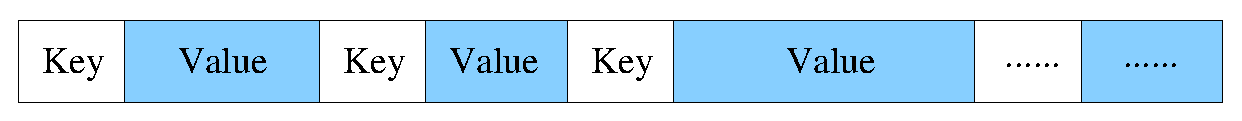
\epsfig{file=sstable.eps,width=1.00\linewidth}
\caption{SSTable}
\label{fig:sstable}
\end{centering}
\end{figure}


We implemented MRIS using LevelDB~\cite{leveldb-web}, an open source
key/value database engine developed by Google. LevelDB is
log-structured and organizes data into Sorted String Table (SSTable).
SSTable, introduced in Bigtable~\cite{chang06osdi}, is an immutable
data structure containing a sequence of key/value pairs sorted by the
key as shown in Figure~\ref{fig:sstable}. Besides key and value, there
might be optional fields such as CRC, compression type etc. SSTable
are mostly saved as files and each of them can contains data
structures, such as bloomfilter, to facilitate key lookup. SSTable
have counterpart in the memory called Memtable. The key/value pairs in
Memtable are often kept in data structures easy for insert and lookup
such as red/black tree and skiplist.

LevelDB, as well as most other key/value engines, use Log-Structured
Merge Trees (LSM)~\cite{lsm} for internal storage. When key/value
pairs are first added, they are inserted into Memtable.  Once the size
of the Memtable growes beyond a certain threshold, the whole Memtable
is flushed out into a SSTable, and a new Memtable is created for
insertion. When key/value pairs get changed, the new pairs are
inserted without modifying the old pairs. When key/value pairs get
deleted, a mark of the deletion is inserted. This way key/value can
provide large insertion throughput because data is written out using
sequential I/Os, which have good performance on Hard Disk Drives
(HDD). 

To serve a key lookup, Memtable is queried firstly. If not found in
Memtable, the SSTables are queried in reverse chronological order. A
naive implementation of such a lookup can be very slow because the
whole database need be read and checked in the worst case. To make
lookup fast, SSTable are organized into several layers with the size
of each table increasing from the top layer to the bottom. Background
jobs are launched periodically to sort and merge small SSTables into
larger ones in the next layer. This is called compaction. Deleted
pairs are also removed during compaction. Then a lookup iterates the
SSTables layer by layer and returns once the key is found.  Because
SSTables are sorted by key, it enables fast lookup algorithm like
binary search. There is also index for SSTables tells the key range
covered by a particular SSTable so that it suffice just checking the
SSTables whose key ranges cover the interested key. Inside each
SSTable, we can have a bloomfilter to filter negative key lookup and a
secondary index for faster search.

In LevelDB, there are two Memtables, once one is filled, the other one
is used for further insertion. The filled one is flushed into a
Memtable in background. Its compaction procedure is illustrated in
Figure~\ref{fig:compact}.

%%%%%%%%%%%%%%%%%%%%%%%%%%%%%%%%%%%%%%%%%%%%%%%%%%%%%%%%%%%%%%%%%%%%%%%%%%%%%%
%% For Emacs:
% Local variables:
% fill-column: 70
% End:
%%%%%%%%%%%%%%%%%%%%%%%%%%%%%%%%%%%%%%%%%%%%%%%%%%%%%%%%%%%%%%%%%%%%%%%%%%%%%%
%% For Vim:
% vim:textwidth=70 noai nocin nosi
%%%%%%%%%%%%%%%%%%%%%%%%%%%%%%%%%%%%%%%%%%%%%%%%%%%%%%%%%%%%%%%%%%%%%%%%%%%%%%
% LocalWords:  SSTable LevelDB Memtables
